\documentclass[tikz,border=12pt]{standalone}
\usepackage{helvet}
\renewcommand{\familydefault}{\sfdefault}
\usepackage{tikz}
\usepackage{amsmath,amssymb}
\usetikzlibrary{shapes.gates.logic.US, shapes.geometric, positioning, calc, arrows.meta}

\definecolor{emeraldpine}{HTML}{1A4D3E}
\definecolor{harvardcrimson}{HTML}{A51C30}
\definecolor{ethdarkblue}{HTML}{1F407A}
\definecolor{ethpetrol}{HTML}{007A87}
\definecolor{ethbronze}{HTML}{B87333}
\definecolor{ink}{HTML}{1A202C}
\definecolor{cardbg}{HTML}{F8FAFC}
\definecolor{shadecolor}{HTML}{F4F6F9}

\begin{document}
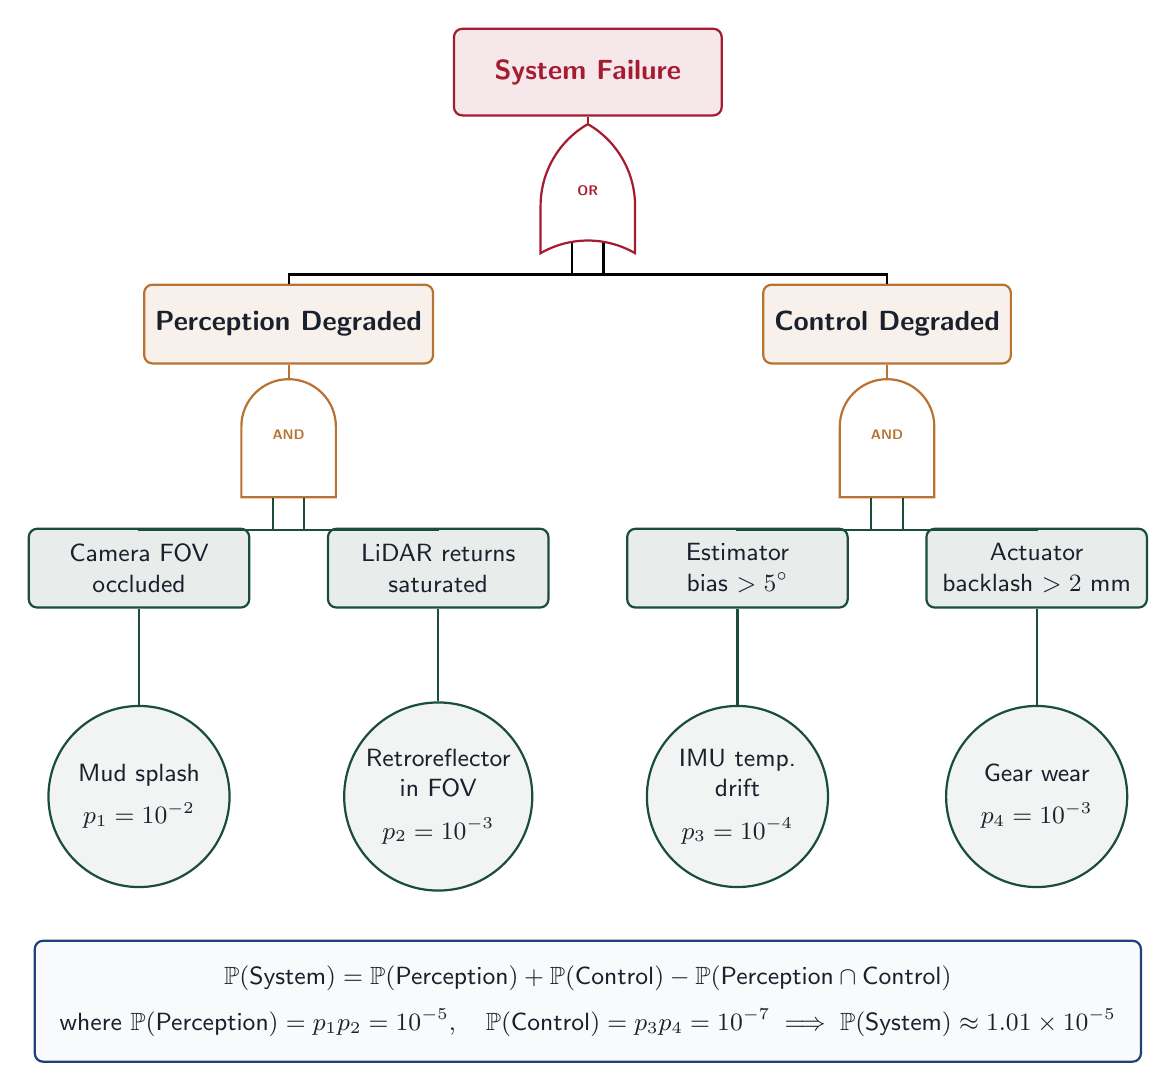
\begin{tikzpicture}[
    >=Stealth,
    font=\small,
    box/.style={draw, rectangle, rounded corners=3pt, align=center, fill=cardbg, text=ink, thick, minimum width=2.8cm, minimum height=1cm, inner sep=4pt},
    event/.style={draw, circle, align=center, fill=shadecolor, text=ink, thick, minimum size=2.3cm, inner sep=2pt},
    line/.style={draw, thick, -}
]

% ── Level 0: Top Event ───────────────────────────────────────────────────
\node[box, draw=harvardcrimson, fill=harvardcrimson!10, text=harvardcrimson, font=\bfseries\normalsize, minimum width=3.4cm, minimum height=1.1cm] 
    (sys) at (0, 0) {System Failure};

% OR gate below Top Event
\node[or gate US, draw=harvardcrimson, thick, rotate=90, minimum size=1.2cm, fill=white] 
    (or1) at (0, -1.6) {};
\node[font=\bfseries\tiny, text=harvardcrimson] at (0, -1.5) {OR};
\draw[line, draw=harvardcrimson, thick] (or1.east) -- (sys.south);

% ── Level 1: Subsystem Degradation (x = -3.8 and +3.8) ───────────────────
\node[box, draw=ethbronze, fill=ethbronze!10, font=\bfseries] 
    (perc) at (-3.8, -3.2) {Perception Degraded};
\node[box, draw=ethbronze, fill=ethbronze!10, font=\bfseries] 
    (ctrl) at (3.8, -3.2) {Control Degraded};

% Clean orthogonal bus wiring into OR gate from below
\draw[line, thick] (perc.north) |- ($(or1.input 2) + (0, -0.4)$) -- (or1.input 2);
\draw[line, thick] (ctrl.north) |- ($(or1.input 1) + (0, -0.4)$) -- (or1.input 1);

% ── AND Gates below Level 1 ──────────────────────────────────────────────
\node[and gate US, draw=ethbronze, thick, rotate=90, minimum size=1.2cm, fill=white] 
    (and1) at (-3.8, -4.7) {};
\node[font=\bfseries\tiny, text=ethbronze] at (-3.8, -4.6) {AND};
\draw[line, draw=ethbronze, thick] (and1.east) -- (perc.south);

\node[and gate US, draw=ethbronze, thick, rotate=90, minimum size=1.2cm, fill=white] 
    (and2) at (3.8, -4.7) {};
\node[font=\bfseries\tiny, text=ethbronze] at (3.8, -4.6) {AND};
\draw[line, draw=ethbronze, thick] (and2.east) -- (ctrl.south);

% ── Level 2: Intermediate Faults (x = -5.7, -1.9, +1.9, +5.7) ───────────
\node[box, draw=emeraldpine, fill=emeraldpine!10] 
    (cam) at (-5.7, -6.3) {Camera FOV\\occluded};
\node[box, draw=emeraldpine, fill=emeraldpine!10] 
    (lidar) at (-1.9, -6.3) {LiDAR returns\\saturated};

\node[box, draw=emeraldpine, fill=emeraldpine!10] 
    (est) at (1.9, -6.3) {Estimator\\bias $> 5^\circ$};
\node[box, draw=emeraldpine, fill=emeraldpine!10] 
    (act) at (5.7, -6.3) {Actuator\\backlash $> 2$ mm};

% Clean orthogonal bus wiring into AND gates from below
\draw[line, draw=emeraldpine, thick] (cam.north) |- ($(and1.input 2) + (0, -0.4)$) -- (and1.input 2);
\draw[line, draw=emeraldpine, thick] (lidar.north) |- ($(and1.input 1) + (0, -0.4)$) -- (and1.input 1);

\draw[line, draw=emeraldpine, thick] (est.north) |- ($(and2.input 2) + (0, -0.4)$) -- (and2.input 2);
\draw[line, draw=emeraldpine, thick] (act.north) |- ($(and2.input 1) + (0, -0.4)$) -- (and2.input 1);

% ── Level 3: Basic Initiating Events (circles) ───────────────────────────
\node[event, draw=emeraldpine, fill=emeraldpine!6] 
    (mud) at (-5.7, -9.2) {Mud splash\\[1.5mm] \textbf{$p_1 = 10^{-2}$}};
\node[event, draw=emeraldpine, fill=emeraldpine!6] 
    (retro) at (-1.9, -9.2) {Retroreflector\\in FOV\\[1.5mm] \textbf{$p_2 = 10^{-3}$}};

\draw[line, draw=emeraldpine, thick] (mud.north) -- (cam.south);
\draw[line, draw=emeraldpine, thick] (retro.north) -- (lidar.south);

\node[event, draw=emeraldpine, fill=emeraldpine!6] 
    (imu) at (1.9, -9.2) {IMU temp.\\drift\\[1.5mm] \textbf{$p_3 = 10^{-4}$}};
\node[event, draw=emeraldpine, fill=emeraldpine!6] 
    (gear) at (5.7, -9.2) {Gear wear\\[1.5mm] \textbf{$p_4 = 10^{-3}$}};

\draw[line, draw=emeraldpine, thick] (imu.north) -- (est.south);
\draw[line, draw=emeraldpine, thick] (gear.north) -- (act.south);

% ── Bottom Math Formula Box ──────────────────────────────────────────────
\node[font=\small, text=ink, align=center, fill=cardbg, draw=ethdarkblue, thick, rounded corners=3pt, inner sep=9pt] 
    at (0, -11.8) {
    $\mathbb{P}(\text{System}) = \mathbb{P}(\text{Perception}) + \mathbb{P}(\text{Control}) - \mathbb{P}(\text{Perception} \cap \text{Control})$ \\[2mm]
    $\text{where } \mathbb{P}(\text{Perception}) = p_1 p_2 = 10^{-5}, \quad \mathbb{P}(\text{Control}) = p_3 p_4 = 10^{-7} \implies \mathbb{P}(\text{System}) \approx 1.01 \times 10^{-5}$
};

\end{tikzpicture}
\end{document}
